% textidote: ignore begin
\subsection{Development}\label{subsec:development}
% textidote: ignore end

Throughout development, several technologies have been used.
The primary reasons for using these are efficiency and productivity.
By taking advantage of these technologies, we leverage the prevalence of existing technologies in our work.

\subsubsection{GitHub}

Most notably, GitHub~\cite{github2024} and several of their features have been used:

\begin{itemize}
    \item \textbf{GitHub:}
    We use GitHub for storing our codebase, both for the report code and application code.
    Team members access these codebases remotely from their own client by using Git~\cite{git2024} and push and pull
    code to the remote repository.
    This makes for safekeeping as well as versioning of the code.
    \item \textbf{GitHub Projects:}
    GitHub Projects enables the team to see all issues for all related repositories in the same window, thereby
    providing an easy oversight of all codebases.
    A visualization of this can be seen in Figure~\ref{fig:github-projects-screenshot}.
    \item \textbf{GitHub Issues:}
    We use GitHub Issues to track what new feature or bug the team members are working on.
    This makes it easy for all team members to see what others are working on as well as enabling them to work together
    on an issue.
    Several examples of issues can be seen in Figure~\ref{fig:github-projects-screenshot}.
    \item \textbf{GitHub Actions:}
    We have several GitHub Actions running in each repository for linting, spell checking, best practices and to
    circumvent errors and bugs.
    This makes it easy to check the code for these beforehand mentioned things without manually having to check for
    them.
    This enables quicker code reviews and more trust in the code, thereby improving productivity and efficiency in
    development.
\end{itemize}

\begin{figure}[h]
    \centering
    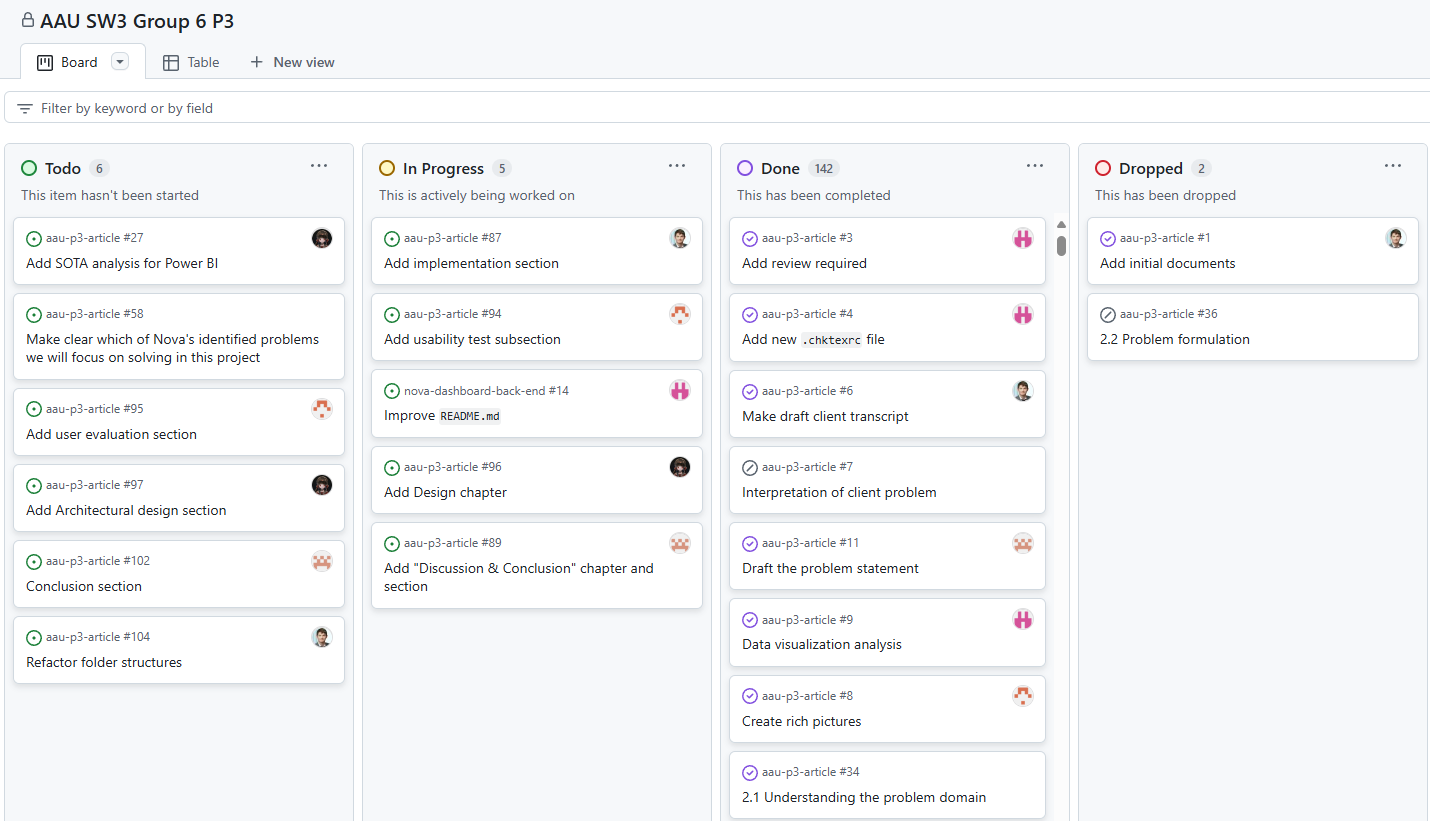
\includegraphics[width=\textwidth]{github-projects-screenshot}
    \caption{A screenshot of the GitHub Project overview during development.
    }\label{fig:github-projects-screenshot}
\end{figure}

% textidote: ignore begin
\subsubsection{Docker}
% textidote: ignore end

Another important technology we have relied on during development, as well as production, is Docker.
Docker handles the hosting of our database as well as hosting the other codebases through containerization.
The technology enables consistency when running the code and works as a sandbox environment.
This makes for fewer bugs overall and thereby less time spent debugging.
